\label{sec:metrics}

Once defined the coding schemes behavior in terms of encoding
and decoding, we proceed to describe the metrics considered in our study.
The goodput is a measure for the effective processing speed since it
excludes protocol overhead but considers all delays related with
algorithmic procedures, field operations, hardware processing, multicore
coordination (where it applies), etc. Moreover, encoding and decoding
goodput permits to observe if coding is a system-block that limits the
end-to-end performance. If a system presents a low goodput, this will
affect the \ac{QoE} of delay-intolerant applications for the end user.
For example, mobile user applications are typically delay-intolerant.
Furthermore, Raspberry Pi processors are based in the \ac{ARM} architecture
which is the same as in mobile devices such as smartphones or tables.
Thus, the Raspberry Pi might be used as an experimental tool to get an
estimate of a mobile device processing capability which is easy-deployable
and at a much lower cost than a smartphone.

To complement our study, we review the energy consumption of the Raspberry
Pi since this platform is deployed at a large scale in scenarios where (i)
energy is constrained to the lifetime of the device battery and (ii) the
devices could be established in locations that are unavailable for
regular maintenance. Typical use cases of this type of scenarios are
sensor applications where devices are positioned for measurement retrieval
without any supervision for large periods fo time.

\subsection{Goodput}
We consider the goodput defined as the ratio of the useful delivered
information at the application layer and the total delivery time. We focus
on the goodput considering only the coding process, i.e. we assume that
the application data has been properly generated before encoding and
also correctly post-processed after decoding. In this way, the goodput



\subsubsection{Encoding}
Encoding benchmark
\begin{figure}[ht!]
\centering
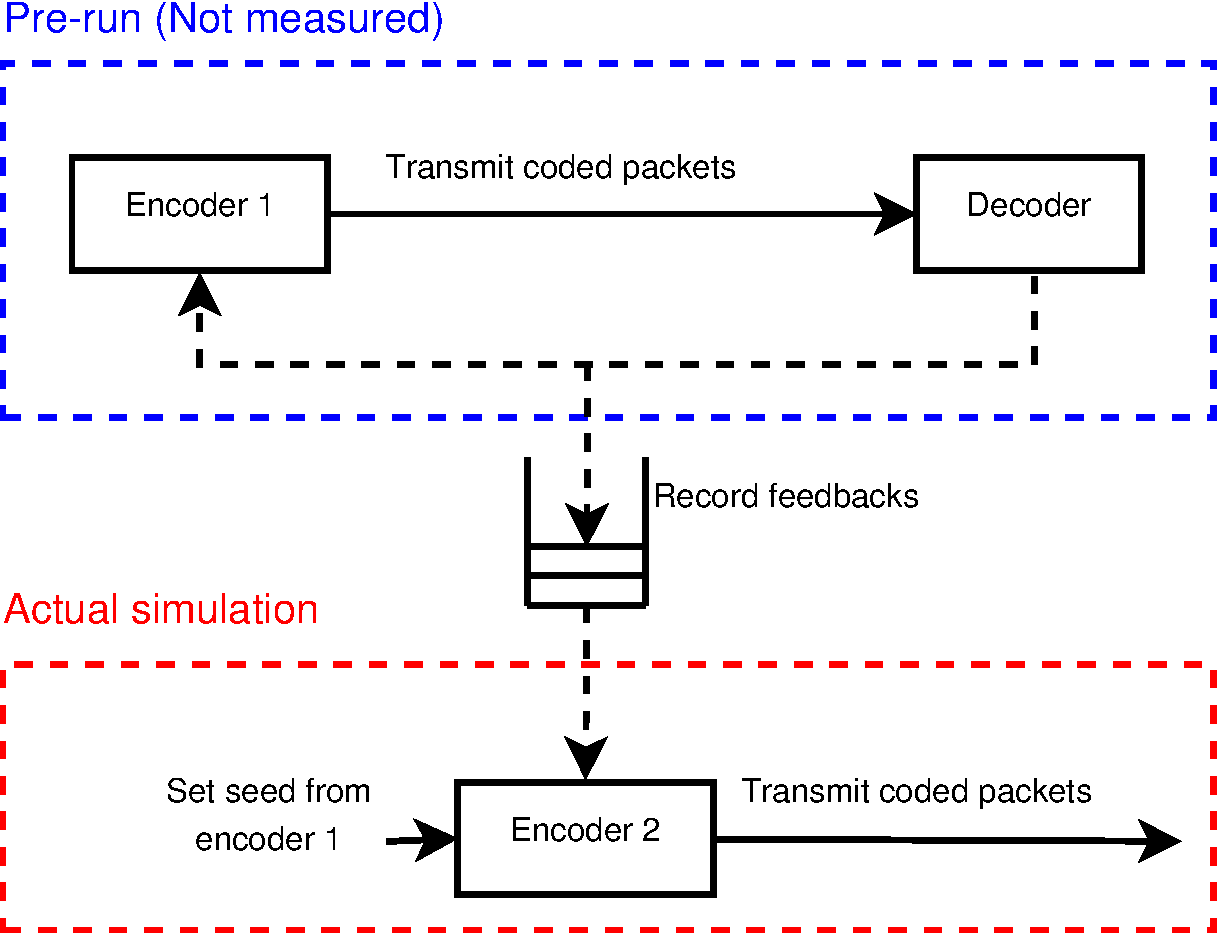
\includegraphics[width=0.6\textwidth]{images/measure_encoder.pdf}
\caption{Encoding goodput benchmark}
\label{fig:enc_goodput_benchmark}
\end{figure}

\subsubsection{Decoding}
Decoding benchmark

\begin{figure}[ht!]
\centering
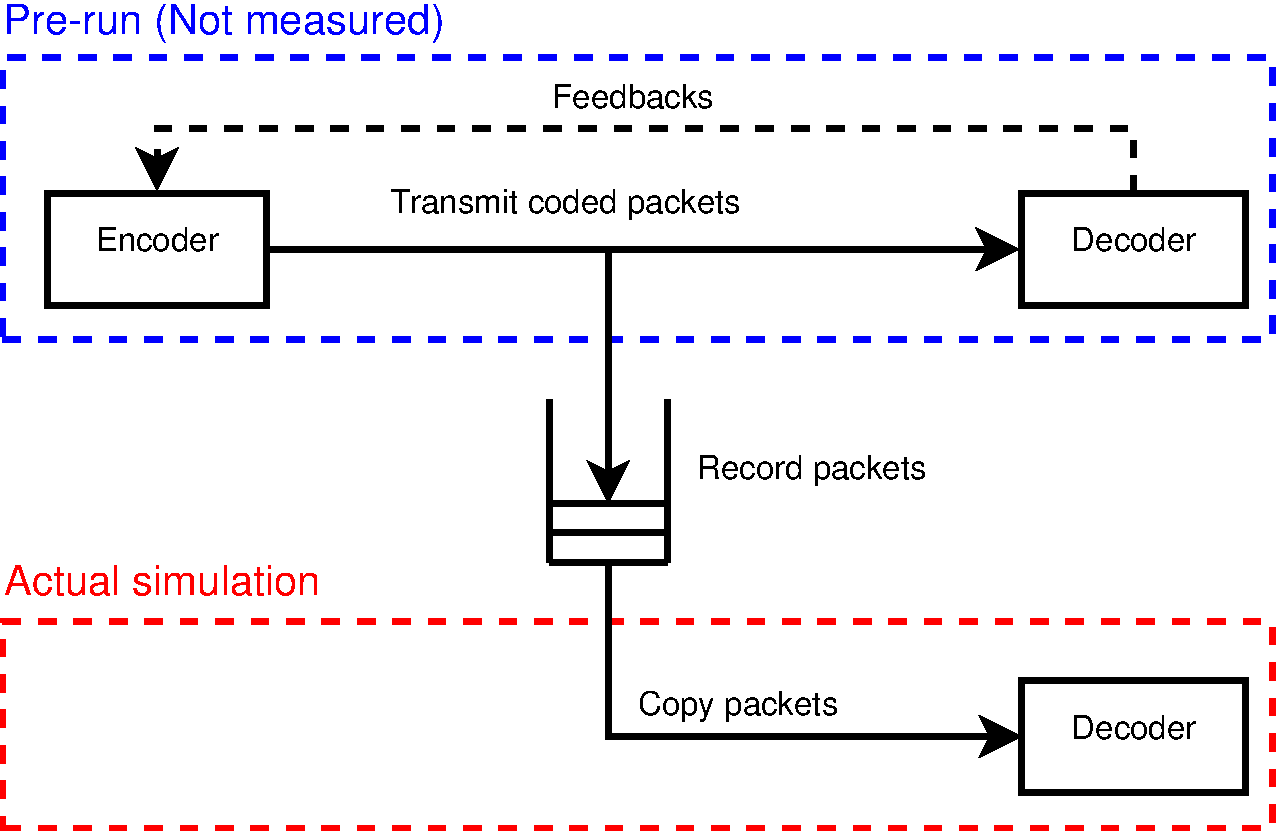
\includegraphics[width=0.6\textwidth]{images/measure_decoder.pdf}
\caption{Decoding goodput benchmark}
\label{fig:dec_goodput_benchmark}
\end{figure}

\subsection{Energy Consumption}
In large-scale networks where several Raspberry Pis might be deployed,
both overall and per-bit energy consumption of the devices during the
encoding and decoding process are relevant parameters that impact in the
network performance for a given coding scheme. To compute the

\subsubsection{Average}
\subsubsection{Per-Bit}